%%%%%%%%%%%%%%%%%%%%%%%%%%%%%%%%%%%%%%%%%
%%% IRD-OB7 Project Reporting Template
%%%%%%%%%%%%%%%%%%%%%%%%%%%%%%%%%%%%%%%%%

\documentclass[11pt]{report}

\usepackage{ird-ob7}		% IRD-OB7 specific definitions and styles  
\usepackage[utf8]{inputenc}	% UTF8 package
\usepackage[T1]{fontenc}
\usepackage{textcomp}		% common special chars
\usepackage{amsmath}		% math formula
\usepackage{fancybox}
\usepackage{anyfontsize}	% fonts
\usepackage{lipsum}
\usepackage{float}
\usepackage[normalem]{ulem}
\usepackage{cleveref}
\usepackage[printonlyused]{acronym}
\hypersetup{
	pdftitle={0th Periodic Report},
	pdfauthor={[Names of co-authors (partners short names)]},
	pdfkeywords={Periodic Report, European Union (EU), H2020, Project, ERIGrid 2.0, GA GA 870620},
}

\graphicspath{ {graphics/} }

%%%%%%%%%%%%%%%%%%%%%%%%%%%%%%%%%%%%%%%%%
%%% Definitions
%%%%%%%%%%%%%%%%%%%%%%%%%%%%%%%%%%%%%%%%%

\def\todo#1{{\color{erigrid2red}\textbf{TODO:} ``#1''}}
\def\teams{IRD-OB7 teams}
\def\disclaimer{All information provided reflects the status of the project at the time of writing and may be subject to change.}

% CHANGE %'s below to make subsection headings visible/invisible in TOC
%\newcommand{\xsubsubsection}[1]{\subsection{#1}}
%\newcommand{\xsubsubsection}[1]{\subsubsection{#1}}

\begin{document}

%%%%%%%%%%%%%%%%%%%%%%%%%%%%%%%%%%%%%%%%%
%%% URL style same as regular text
%%%%%%%%%%%%%%%%%%%%%%%%%%%%%%%%%%%%%%%%%
	
\urlstyle{same}

%%%%%%%%%%%%%%%%%%%%%%%%%%%%%%%%%%%%%%%%%
%%% Deliverable Information
%%%%%%%%%%%%%%%%%%%%%%%%%%%%%%%%%%%%%%%%%

% Project Meta Information
\ProjectFullTitle{European Research Infrastructure supporting Smart Grid and Smart Energy Systems Research, Technology Development, Validation and Roll Out -- Second Edition}
\ProjectAcronym{ERIGrid 2.0}
\ProjectRefNo{870620}

% Report Number, use either "1", "2", or "3" for the corresponding reporting period
\delivNumber{0}

% Period covered by the report
\delivFrom{dd/mm/yyyy}
\delivTo{dd/mm/yyyy}

% Report Responsible Partner
\delivResponsible{AIT Austrian Institute of Technology (AIT)} 

% Report Version, Contractual and Actual Date, Dissemination Level, Type
\delivVersion{vn.n}
\ContractualDate{dd/mm/yyyy}
\ActualDate{dd/mm/yyyy}

% List of Main Authors (usually from the responsible partner)
\delivAuthor{[Names of co-authors (partners short names)]}

% List of Co-Authors (all other co-authors should be listed here)
\delivFPAuthor{[Names of co-authors (partners short names)]}

% Report Status
\delivStatus{d} %% d = draft, f = final, s = submitted

%%%%%%%%%%%%%%%%%%%%%%%%%%%%%%%%%%%%%%%%%
%%% Change Log
%%%%%%%%%%%%%%%%%%%%%%%%%%%%%%%%%%%%%%%%%

\istChange{dd/mm/yyyy}{v1.0}{Name (Partner short name)}{Draft report template}
\istChange{}{}{}{}

%%%%%%%%%%%%%%%%%%%%%%%%%%%%%%%%%%%%%%%%%
%%% Cover Page
%%%%%%%%%%%%%%%%%%%%%%%%%%%%%%%%%%%%%%%%%

\makecover

%%%%%%%%%%%%%%%%%%%%%%%%%%%%%%%%%%%%%%%%%
%%% Table of Contents
%%%%%%%%%%%%%%%%%%%%%%%%%%%%%%%%%%%%%%%%%

\clearpage
\fancypagestyle{plain}{}
\settableofcontents
\tableofcontents

%%%%%%%%%%%%%%%%%%%%%%%%%%%%%%%%%%%%%%%%%
%%% List of Figures
%%%%%%%%%%%%%%%%%%%%%%%%%%%%%%%%%%%%%%%%%

\clearpage
\setlistoffigures
\listoffigures

%%%%%%%%%%%%%%%%%%%%%%%%%%%%%%%%%%%%%%%%%
%%% List of Tables
%%%%%%%%%%%%%%%%%%%%%%%%%%%%%%%%%%%%%%%%%

\clearpage
\setlistoftables
\listoftables

%%%%%%%%%%%%%%%%%%%%%%%%%%%%%%%%%%%%%%%%%
%%% List of Abbreviations
%%%%%%%%%%%%%%%%%%%%%%%%%%%%%%%%%%%%%%%%%

%%%%%%%%%%%%%%%%%%%%%%%%%%%%%%%%%%%%%%%%%
%%% List of Abbreviations
%%%%%%%%%%%%%%%%%%%%%%%%%%%%%%%%%%%%%%%%%

\clearpage
\section*{List of Abbreviations}
\label{sec:abbreviations}

\begin{acronym}[ABCDEF]
	\acro{DMP}{Data Management Plan}
	\acro{DoA}{Description of Action}
	\acro{DoI}{Digital Object Identifier}
	\acro{EU}{European Union}
	\acro{GA}{Grant Agreement}
	\acro{OA}{Open Access}
	\acro{RI}{Research Infrastructure}
	\acro{RP}{Reporting Period}
	\acro{PM}{Person Month}
	\acro{TA}{Trans-national Access Activities}
	\acro{VA}{Virtual Access Activities}
	\acro{WP}{Work Package}
\end{acronym}

%%%%%%%%%%%%%%%%%%%%%%%%%%%%%%%%%%%%%%%%%

%%%%%%%%%%%%%%%%%%%%%%%%%%%%%%%%%%%%%%%%%
%%% Deliverable Content
%%%%%%%%%%%%%%%%%%%%%%%%%%%%%%%%%%%%%%%%%

%%%%%%%%%%%%%%%%%%%%%%%%%%%%%%%%%%%%%%%%%
%%% Explanation of the Work carried out
%%% by the Beneficiaries and Overview of 
%%% the Progress
%%%%%%%%%%%%%%%%%%%%%%%%%%%%%%%%%%%%%%%%%

\clearpage
\section{Explanation of the Work carried out by the Beneficiaries and Overview of the Progress}
\label{sec:work-carried-out}

%%%%%%%%%%%%%%%%%%%%%%%%%%%%%%%%%%%%%%%%%
%%% Section content, please change!
%%%%%%%%%%%%%%%%%%%%%%%%%%%%%%%%%%%%%%%%%

This section summarises the work carried out by the \erigrid2 consortium during the \nth{0} \ac{RP} towards the project goals and work plan as described in the \ac{GA} \cite{bib:grantagreement2019}. 

\subsection{Objectives}

\todo{List the specific objectives for the project as described in Section 1.1 of the \ac{DoA} and described the work carried out during the reporting period towards the achievement of each listed objective. Provide clear and measurable details.}

\subsection{Explanation of the Work Carried per \acl{WP}}

This section provides an overview of the work carried out and results achieved per \ac{WP} 
during the the \nth{0} \acl{RP}.   

%%%%%%%%%%%%%%%%%%%%%%%%%%%%%%%%%%%%%%%%%
%%% WP01
%%%%%%%%%%%%%%%%%%%%%%%%%%%%%%%%%%%%%%%%%

\subsubsection{\acl{WP} WP01}

%%%%%%%%%%%%%%%%%%%%%%%%%%%%%%%%%%%%%%%%%
%%% Section content, please change!
%%%%%%%%%%%%%%%%%%%%%%%%%%%%%%%%%%%%%%%%%

\paragraph{Overview and Goals} \mbox{}

\begin{table}[H]
    \renewcommand{\arraystretch}{1.50}		
    \footnotesize   
    \begin{tabular}{*{3}{|p{0.10\textwidth}}|l|}
        \hline
        \rowcolor{erigrid2gray} \multicolumn{4}{|c|}{\textit{\color{white}Work Package Summary}} \\
        \hline
        \rowcolor{erigrid2lightergray} \textit{WP No.} & \cellcolor{white} 01 & \textit{Title of WP} & \cellcolor{white} WP Title \\
        \hline
        \rowcolor{erigrid2lightergray} \textit{Start} & \cellcolor{white} Mxx & \textit{End} & \cellcolor{white} Myy \\
        \hline
        \rowcolor{erigrid2lightergray} \multicolumn{4}{|p{0.978\textwidth}|}{\textit{Participating Organisations}} \\
        \hline
        \multicolumn{4}{|p{0.978\textwidth}|}{
            \hspace*{-0.75cm} 
            \begin{minipage}[t]{\textwidth}
    			\begin{itemize}
    			    \item WP Leader: Partner 1
    				\item Participants: Partner 2, Partner 3, Partner 4, Partner 5, Partner 6, Partner 7
    			\end{itemize} 
    			\vspace*{0.10em}
			\end{minipage}
        } \\
        \hline
    \end{tabular}
    \vspace{0.5em}\vfill
    \begin{tabular}{|p{0.978\textwidth}|}
        \hline
        \rowcolor{erigrid2lightergray} \textit{Goals} \\
        \hline
        \rowcolor{white} 
        \hspace*{-0.75cm} 
        \begin{minipage}[t]{\textwidth}
    		\begin{itemize}
    		    \item Goal 1
    			\item Goal 2
			    \item Goal 3
    		\end{itemize} 
    		\vspace*{0.10em}
		\end{minipage}        
        \\
        \hline
    \end{tabular}
    \vspace{0.5em}\vfill
    \begin{tabular}{|l|*{7}{>{\centering\arraybackslash}p{0.084\textwidth}|}}
        \hline    
        \rowcolor{erigrid2lightergray} \textit{Participant number} & \textit{1} & \textit{2} & \textit{3} & \textit{4} & \textit{5} & \textit{6} & \textit{7} \\
        \hline
        \rowcolor{white} \cellcolor{erigrid2lightergray}\textit{Participant short name} & Partner 1 & Partner 2 & Partner 3 & Partner 4 & Partner 5 & Partner 6 & Partner 7 \\
        \hline
        \rowcolor{white} \cellcolor{erigrid2lightergray}\textit{PM per participant} & xx & xx & xx & xx & xx & xx & xx \\
        \hline        
    \end{tabular}    
\end{table}

\paragraph{Status} \mbox{}

\todo{Briefly explain the status of the \ac{WP}.}

\paragraph{Progress per Task} \mbox{}

\subparagraph{Task no: title (Month xx-yy)} \mbox{}

\todo{Briefly explain the progress of the task in context to the \ac{DoA}.}

\subparagraph{Task no: title (Month xx-yy)} \mbox{}

\todo{Briefly explain the progress of the task in context to the \ac{DoA}.}

\paragraph{Main Results and Achievements} \mbox{}

\todo{Briefly summarise the main results and achievements of the \ac{WP} in context of the \ac{DoA}.}

\paragraph{Deviations and Corrective Actions} \mbox{}

\todo{Briefly summarise any deviations and performed corrective actions of the \ac{WP} in context of the \ac{DoA}.}

%%%%%%%%%%%%%%%%%%%%%%%%%%%%%%%%%%%%%%%%%
%%%%%%%%%%%%%%%%%%%%%%%%%%%%%%%%%%%%%%%%%
%%% WP02
%%%%%%%%%%%%%%%%%%%%%%%%%%%%%%%%%%%%%%%%%

\subsubsection{\acl{WP} WP02}

%%%%%%%%%%%%%%%%%%%%%%%%%%%%%%%%%%%%%%%%%
%%% Section content, please change!
%%%%%%%%%%%%%%%%%%%%%%%%%%%%%%%%%%%%%%%%%

\paragraph{Overview and Goals} \mbox{}

\begin{table}[H]
    \renewcommand{\arraystretch}{1.50}		
    \footnotesize   
    \begin{tabular}{*{3}{|p{0.10\textwidth}}|l|}
        \hline
        \rowcolor{erigrid2gray} \multicolumn{4}{|c|}{\textit{\color{white}Work Package Summary}} \\
        \hline
        \rowcolor{erigrid2lightergray} \textit{WP No.} & \cellcolor{white} 02 & \textit{Title of WP} & \cellcolor{white} WP Title \\
        \hline
        \rowcolor{erigrid2lightergray} \textit{Start} & \cellcolor{white} Mxx & \textit{End} & \cellcolor{white} Myy \\
        \hline
        \rowcolor{erigrid2lightergray} \multicolumn{4}{|p{0.978\textwidth}|}{\textit{Participating Organisations}} \\
        \hline
        \multicolumn{4}{|p{0.978\textwidth}|}{
            \hspace*{-0.75cm} 
            \begin{minipage}[t]{\textwidth}
    			\begin{itemize}
    			    \item WP Leader: Partner 1
    				\item Participants: Partner 2, Partner 3, Partner 4, Partner 5, Partner 6, Partner 7
    			\end{itemize} 
    			\vspace*{0.10em}
			\end{minipage}
        } \\
        \hline
    \end{tabular}
    \vspace{0.5em}\vfill
    \begin{tabular}{|p{0.978\textwidth}|}
        \hline
        \rowcolor{erigrid2lightergray} \textit{Goals} \\
        \hline
        \rowcolor{white} 
        \hspace*{-0.75cm} 
        \begin{minipage}[t]{\textwidth}
    		\begin{itemize}
    		    \item Goal 1
    			\item Goal 2
			    \item Goal 3
    		\end{itemize} 
    		\vspace*{0.10em}
		\end{minipage}        
        \\
        \hline
    \end{tabular}
    \vspace{0.5em}\vfill
    \begin{tabular}{|l|*{7}{>{\centering\arraybackslash}p{0.084\textwidth}|}}
        \hline    
        \rowcolor{erigrid2lightergray} \textit{Participant number} & \textit{1} & \textit{2} & \textit{3} & \textit{4} & \textit{5} & \textit{6} & \textit{7} \\
        \hline
        \rowcolor{white} \cellcolor{erigrid2lightergray}\textit{Participant short name} & Partner 1 & Partner 2 & Partner 3 & Partner 4 & Partner 5 & Partner 6 & Partner 7 \\
        \hline
        \rowcolor{white} \cellcolor{erigrid2lightergray}\textit{PM per participant} & xx & xx & xx & xx & xx & xx & xx \\
        \hline        
    \end{tabular}    
\end{table}

\paragraph{Status} \mbox{}

\todo{Briefly explain the status of the \ac{WP}.}

\paragraph{Progress per Task} \mbox{}

\subparagraph{Task no: title (Month xx-yy)} \mbox{}

\todo{Briefly explain the progress of the task in context to the \ac{DoA}.}

\subparagraph{Task no: title (Month xx-yy)} \mbox{}

\todo{Briefly explain the progress of the task in context to the \ac{DoA}.}

\paragraph{Main Results and Achievements} \mbox{}

\todo{Briefly summarise the main results and achievements of the \ac{WP} in context of the \ac{DoA}.}

\paragraph{Deviations and Corrective Actions} \mbox{}

\todo{Briefly summarise any deviations and performed corrective actions of the \ac{WP} in context of the \ac{DoA}.}

%%%%%%%%%%%%%%%%%%%%%%%%%%%%%%%%%%%%%%%%%
%%%%%%%%%%%%%%%%%%%%%%%%%%%%%%%%%%%%%%%%%
%%% WPxy
%%%%%%%%%%%%%%%%%%%%%%%%%%%%%%%%%%%%%%%%%

\subsubsection{\acl{WP} WPxy}

%%%%%%%%%%%%%%%%%%%%%%%%%%%%%%%%%%%%%%%%%
%%% Section content, please change!
%%%%%%%%%%%%%%%%%%%%%%%%%%%%%%%%%%%%%%%%%

\paragraph{Overview and Goals} \mbox{}

\begin{table}[H]
    \renewcommand{\arraystretch}{1.50}		
    \footnotesize   
    \begin{tabular}{*{3}{|p{0.10\textwidth}}|l|}
        \hline
        \rowcolor{erigrid2gray} \multicolumn{4}{|c|}{\textit{\color{white}Work Package Summary}} \\
        \hline
        \rowcolor{erigrid2lightergray} \textit{WP No.} & \cellcolor{white} xy & \textit{Title of WP} & \cellcolor{white} WP Title \\
        \hline
        \rowcolor{erigrid2lightergray} \textit{Start} & \cellcolor{white} Mxx & \textit{End} & \cellcolor{white} Myy \\
        \hline
        \rowcolor{erigrid2lightergray} \multicolumn{4}{|p{0.978\textwidth}|}{\textit{Participating Organisations}} \\
        \hline
        \multicolumn{4}{|p{0.978\textwidth}|}{
            \hspace*{-0.75cm} 
            \begin{minipage}[t]{\textwidth}
    			\begin{itemize}
    			    \item WP Leader: Partner 1
    				\item Participants: Partner 2, Partner 3, Partner 4, Partner 5, Partner 6, Partner 7
    			\end{itemize} 
    			\vspace*{0.10em}
			\end{minipage}
        } \\
        \hline
    \end{tabular}
    \vspace{0.5em}\vfill
    \begin{tabular}{|p{0.978\textwidth}|}
        \hline
        \rowcolor{erigrid2lightergray} \textit{Goals} \\
        \hline
        \rowcolor{white} 
        \hspace*{-0.75cm} 
        \begin{minipage}[t]{\textwidth}
    		\begin{itemize}
    		    \item Goal 1
    			\item Goal 2
			    \item Goal 3
    		\end{itemize} 
    		\vspace*{0.10em}
		\end{minipage}        
        \\
        \hline
    \end{tabular}
    \vspace{0.5em}\vfill
    \begin{tabular}{|l|*{7}{>{\centering\arraybackslash}p{0.084\textwidth}|}}
        \hline    
        \rowcolor{erigrid2lightergray} \textit{Participant number} & \textit{1} & \textit{2} & \textit{3} & \textit{4} & \textit{5} & \textit{6} & \textit{7} \\
        \hline
        \rowcolor{white} \cellcolor{erigrid2lightergray}\textit{Participant short name} & Partner 1 & Partner 2 & Partner 3 & Partner 4 & Partner 5 & Partner 6 & Partner 7 \\
        \hline
        \rowcolor{white} \cellcolor{erigrid2lightergray}\textit{PM per participant} & xx & xx & xx & xx & xx & xx & xx \\
        \hline        
    \end{tabular}    
\end{table}

\paragraph{Status} \mbox{}

\todo{Briefly explain the status of the \ac{WP}.}

\paragraph{Progress per Task} \mbox{}

\subparagraph{Task no: title (Month xx-yy)} \mbox{}

\todo{Briefly explain the progress of the task in context to the \ac{DoA}.}

\subparagraph{Task no: title (Month xx-yy)} \mbox{}

\todo{Briefly explain the progress of the task in context to the \ac{DoA}.}

\paragraph{Main Results and Achievements} \mbox{}

\todo{Briefly summarise the main results and achievements of the \ac{WP} in context of the \ac{DoA}.}

\paragraph{Deviations and Corrective Actions} \mbox{}

\todo{Briefly summarise any deviations and performed corrective actions of the \ac{WP} in context of the \ac{DoA}.}

%%%%%%%%%%%%%%%%%%%%%%%%%%%%%%%%%%%%%%%%%

\subsection{Impact}

\todo{Include in this section whether the information on section 2.1 of the DoA  (how your project will contribute to the expected impacts) is still relevant or needs to be updated. Include further details in the latter case.}

\subsection{Access Provisions to \aclp{RI}}

\subsubsection{\acl{TA}}

\paragraph{Description of the publicity concerning the new opportunities for access} \mbox{}

\todo{In the first periodic report describe the measures taken to publicise to research teams throughout Europe the opportunities for access open to them under the \ac{GA}. In the following periodic reports indicate only additional measures and changes.}

\paragraph{Description of the selection process} \mbox{}

\todo{In the first periodic report, describe the procedure used to select users: organisation of the Selection Panel, any additional selection criteria  employed by the Selection Panel, measures to promote equal opportunities, etc. Specify if feedback is given to rejected applicants and in which form. In the following periodic reports indicate only changes to the existing procedure.\\[0.5em]
The list of the Selection Panel members should be maintained and update when necessary in order to prove that the panel is composed following the conditions indicated in Article 16.1 of the \ac{GA}. The Commission reserves the right to request this list at any time.\\[0.5em]
Indicate number, date and venue (if not carried out remotely) of the meetings of the Selection panel during the reporting period.\\[0.5em]
Provide integrated information on the selection of user projects and on the scientific output of supported users. In particular  indicate the number of eligible User projects submitted in the reporting period and the number of the selected ones taking into account only calls for which the selection has been completed in the reporting period. Indicate also the number of user projects, started and supported in the reporting period, which have a majority of users not working in an \ac{EU} or associated country.}

\paragraph{Description of \ac{TA}} \mbox{}

\todo{Give an overview of the user-projects  and users supported in the reporting period indicating their number, their scientific fields and other relevant information you may want to highlight. You should maintain the list of the user-projects for which costs have been incurred in the reporting period. A user-project can run over more than one reporting period. In this case it should be inserted in the list of each concerned reporting period.\\[0.5em] 
The list of user-projects must include, for each user-project, the acronym, objectives, as well as the amount of access granted to it on each installation used by the user-project in the reporting period. When the user-project is completed in the reporting period the list should also include a short description of the work carried out. The Commission reserves the right to request this list at any time.\\[0.5em]
In addition you must fill the following tables (in Part A to be filled in the IT tool):
\begin{itemize}
    \item List of users:  Researchers who have access to \acp{RI}/installations (one or more) through Union support under the grant either in person (through visit) or through remote access; 
    \item \acp{RI} made accessible to all researchers in Europe and beyond through EU support and summary of trans-national access provision per installation per reporting period indicate for each installation providing trans-national access under the project the quantity of access actually provided in the Reporting Period (expressed in the unit of access defined in Annex 1 for that specific installation). 
\end{itemize}
}

\paragraph{Scientific output of the users at the facilities} \mbox{}

\todo{Give highlights of important research results from the user-projects supported under the grant agreement. Indicate the number and the type of publications derived by user-projects supported under the grant taking into account only publications that acknowledge the support of this \ac{EU} grant.\\[0.5em]
You should maintain a list of publications that have appeared in journals (or conference proceedings) during the reporting period and are resulting from work carried out under the \ac{TA} activity. List only publications that acknowledge the support of the European Community. For each publication indicate: the acronyms of the user-projects that have led to the publication itself, the authors, the title, the year of publication, the type of publication (Article in journal, Publication in conference proceeding/workshop, Book/Monograph, Chapters in book, Thesis/dissertation, whether it has been peer-reviewed or not, the \ac{DoI}, the publication references, and whether the publication is available under \ac{OA} or not. The Commission reserves the right to request this list at any time. 
}

\paragraph{User meetings} \mbox{}

\todo{If any user meetings have been organised in the reporting period, indicate for each of them the date, the venue, the number of users attending the meeting and the overall number of attendees.}

\subsubsection{\acl{VA}}

\todo{Provide statistics on the \ac{VA} in the period by each installation, including quantity, geographical distribution of users and, whenever possible, information/statistics on scientific outcomes (publications, patents, etc.) acknowledging the use of the infrastructure.\\[0.5em]
As indicated in Art. 16.2, the access providers must have the \ac{VA} services assessed periodically by a board composed of international experts in the field, at least half of whom must be independent from the beneficiaries. In the first periodic report, describe how the virtual access providers will comply with this obligation. In the following periodic reports indicate only changes to the existing procedure.\\[0.5em]
When an assessment is scheduled under the reporting period, the assessment report must be submitted as deliverable. 
}

\subsection{Resources used to provide Access to \aclp{RI}}   

\todo{For virtual or trans-national access costs reported as actual costs include, for each access provider, information on how many of the \acp{PM} reported in the use of resources linked to the financial statements have been used to provide access and explain for which task (e.g. scientific support to users, \dots).\\[0.5em]
Information on individual subcontracts must be reported in the use of resources linked to the financial statements in the IT tool. Please mention in the comments field of each subcontract whether it is related to \ac{VA} or \ac{TA}. In addition, all other direct costs items related to virtual or trans-national access must be detailed in the use of resources linked to the financial statements in the IT tool, even if they do not exceed 15\% of personnel costs.}

%%%%%%%%%%%%%%%%%%%%%%%%%%%%%%%%%%%%%%%%%
%%%%%%%%%%%%%%%%%%%%%%%%%%%%%%%%%%%%%%%%%
%%% Update of the Plan for Exploitation and Dissemination of Results
%%%%%%%%%%%%%%%%%%%%%%%%%%%%%%%%%%%%%%%%%

\clearpage
\section{Update of the Plan for Exploitation and Dissemination of Results}
\label{sec:exploitation-dissemination}

%%%%%%%%%%%%%%%%%%%%%%%%%%%%%%%%%%%%%%%%%
%%% Section content, please change!
%%%%%%%%%%%%%%%%%%%%%%%%%%%%%%%%%%%%%%%%%

\todo{Include in this section whether the plan for exploitation and dissemination of results as described in the \ac{DoA} needs to be updated and give details.}

%%%%%%%%%%%%%%%%%%%%%%%%%%%%%%%%%%%%%%%%%
%%%%%%%%%%%%%%%%%%%%%%%%%%%%%%%%%%%%%%%%%
%%% Update of the Data Management Plan
%%%%%%%%%%%%%%%%%%%%%%%%%%%%%%%%%%%%%%%%%

\clearpage
\section{Update of the Data Management Plan}
\label{sec:data-management}

%%%%%%%%%%%%%%%%%%%%%%%%%%%%%%%%%%%%%%%%%
%%% Section content, please change!
%%%%%%%%%%%%%%%%%%%%%%%%%%%%%%%%%%%%%%%%%

\todo{Include in this section whether the \ac{DMP} as described in the \ac{DoA} needs to be updated and give details.}

%%%%%%%%%%%%%%%%%%%%%%%%%%%%%%%%%%%%%%%%%
%%%%%%%%%%%%%%%%%%%%%%%%%%%%%%%%%%%%%%%%%
%%% Follow-up of Recommendations and 
%%% Comments from Previous Review(s) 
%%%%%%%%%%%%%%%%%%%%%%%%%%%%%%%%%%%%%%%%%

\clearpage
\section[Follow-up of Recommendations and Comments from Previous Review(s)]{\texorpdfstring{Follow-up of Recommendations and Comments\\from Previous Review(s)}{Follow-up of Recommendations and Comments from Previous Review(s)}}
\label{sec:follow-up-reviews}

%%%%%%%%%%%%%%%%%%%%%%%%%%%%%%%%%%%%%%%%%
%%% Section content, please change!
%%%%%%%%%%%%%%%%%%%%%%%%%%%%%%%%%%%%%%%%%

\todo{Include in this section the list of recommendations and comments from previous reviews and give information on how they have been followed up.}

%%%%%%%%%%%%%%%%%%%%%%%%%%%%%%%%%%%%%%%%%
%%%%%%%%%%%%%%%%%%%%%%%%%%%%%%%%%%%%%%%%%
%%% Deviations from Annex 1 and Annex 2
%%%%%%%%%%%%%%%%%%%%%%%%%%%%%%%%%%%%%%%%%

\clearpage
\section{Deviations from Annex 1 and Annex 2}
\label{sec:deviations}

%%%%%%%%%%%%%%%%%%%%%%%%%%%%%%%%%%%%%%%%%
%%% Section content, please change!
%%%%%%%%%%%%%%%%%%%%%%%%%%%%%%%%%%%%%%%%%

\subsection{Tasks}

\todo{Include explanations for tasks not fully implemented, critical objectives not fully achieved and/or not being on schedule. Explain also the impact on other tasks on the available resources and the planning.}

\subsection{Use of Resources}

\todo{Include explanations on deviations of the use of resources between actual and planned use of resources in Annex 1, especially related to \acp{PM} per \ac{WP}.\\[0.5em]
Include explanations on transfer of costs categories (if applicable).\\[0.5em]
Include explanations on adjustments to previous financial statements (if applicable).}

\subsubsection{Unforeseen Subcontracting}

\todo{Specify in this section: 
\begin{itemize}
    \item the work (the tasks) performed by a subcontractor which may cover only a limited part of the project;
    \item explanation of the circumstances which caused  the need for a subcontract, taking into account the specific characteristics of the project;
    \item the confirmation that the subcontractor has been selected ensuring the best value for money or, if appropriate, the lowest price and avoiding any conflict of interests.
\end{itemize}
}

\subsubsection{Unforeseen use of in Kind Contribution from Third Party against Payment or Free of 
Charges}

\todo{Specify in this section: 
\begin{itemize}
    \item the identity of the third party;
    \item the resources made available by the third party respectively against payment or free of charges 
    \item explanation of the circumstances which caused  the need for using these resources for carrying out the work.
\end{itemize}
}

%%%%%%%%%%%%%%%%%%%%%%%%%%%%%%%%%%%%%%%%%

%%%%%%%%%%%%%%%%%%%%%%%%%%%%%%%%%%%%%%%%%
%%% References
%%%%%%%%%%%%%%%%%%%%%%%%%%%%%%%%%%%%%%%%%

\clearpage
\bibliography{literature/references}
\bibliographystyle{apacite}

%%%%%%%%%%%%%%%%%%%%%%%%%%%%%%%%%%%%%%%%%
%%% Appendix
%%%%%%%%%%%%%%%%%%%%%%%%%%%%%%%%%%%%%%%%%

\appendix

%%%%%%%%%%%%%%%%%%%%%%%%%%%%%%%%%%%%%%%%%
%%% Appendix A. Document Guidelines
%%%%%%%%%%%%%%%%%%%%%%%%%%%%%%%%%%%%%%%%%

\clearpage
\section*{Appendix A. Document Guidelines}
\addcontentsline{toc}{section}{Appendix A. Document Guidelines}
\label{sec:appendix-a}

%%%%%%%%%%%%%%%%%%%%%%%%%%%%%%%%%%%%%%%%%
%%% Section content, please change!
%%%%%%%%%%%%%%%%%%%%%%%%%%%%%%%%%%%%%%%%%

\subsection*{A.1. Report Titles}
\label{sec:appendix-a1-report-titles}
\addcontentsline{toc}{subsection}{A.1. Report Titles}

Deliverables have a title that is defined in the \ac{DoA}. This title is referred to as the full title of the deliverable. Please stick to the official spelling. It has turned out useful to also have a short title (max 60 characters) for each deliverable, as it can be cumbersome if one always has to use the full title. 

\subsection*{A.2. File Naming}
\label{sec:appendix-a2-file-naming}
\addcontentsline{toc}{subsection}{A.2. File Naming}

The project will generate many documents (deliverable reports) and versions of these reports. It is beneficial to consistently use an agreed file naming format. 

\textit{ERIGrid2-Dnn-ShortTitle-Status-vn.n.Extension}

\begin{itemize}
	\item Notice the hyphen between the various elements of the file name.
    \item {\bf \teams}: Each \teams report should be preceded by the project acronym. Notice, there is only one correct spelling of the acronym: ‘\teams’. 
    \item {\bf Dn.n}: Indicates the deliverable identifier, e.g., ‘D34’ for ‘D3.4’ following the numbering of the \ac{DoA} (Part A of Annex 1 of the Grant Agreement). Notice, there is no dot between the two parts of the deliverable number.
    \item {\bf ShortTitle}: This should be based on the formal short title of deliverables but ‘contracted’ into a single (no spaces) character string using Java class naming convention, e.g., ‘ExploitationPlan’,  or ‘ProjectWebSite’. Avoid underscore, space and other unusual characters.
	\item {\bf Status}: 
	\begin{itemize}
		\item \textit{draft} = Draft Version – indicates that the drafting of the report is in progress; 
		\item \textit{final} = Final Version as checked and updated by the reviewers/WP leader/quality manager; 
		\item \textit{submitted} = submitted version as submitted to the EC by the project coordinator/administrator.
	\end{itemize}
	\item {\bf vn.n}: The version of the report starting from v1.0. 
    \item {\bf Extension}: File extension, e.g., ‘docx’ for Microsoft Word and ‘pdf’ for Portable Document Format. 
\end{itemize}

Examples:

\begin{itemize}
    \item ERIGrid2-D82-InternalCommunication-draft-v1.0.docx
    \item ERIGrid2-D84-QualityAssurancePlan-submitted.pdf
\end{itemize}

\subsection*{A.3. Change Log}
\label{sec:appendix-a3-change-log}
\addcontentsline{toc}{subsection}{A.3. Change Log}

The Change Log is there to keep track of the changes made to the document. Whenever changes are made to the document, a new version should be created and the changes should be briefly summarised in the Change Log. We anticipate a minimum of three phases of Change Log entries. (1) The researcher responsible for the given Deliverable enters the changes as he/she develops the document. (2) The two reviewers register the changes made in the quality assurance phase. Once the responsible researcher passes the report on to the Project Coordinator, the status should be changed from ‘draft’ to ‘final’. (3) The Project Coordinator submits the report to the EC, the status should be changed from ‘final’ to ‘submitted’.

\subsection*{A.4. Document Formatting}
\label{sec:appendix-a4-document-formatting}
\addcontentsline{toc}{subsection}{A.4. Document Formatting}

\subsubsection*{A.4.1. Headings}
\label{sec:appendix-a41-headings}

Like in many journals and books, it is a good practice not to use more than 3 levels of headings. If you really need more, then by all means do so, but you may first consider how to structure the document with a maximum of three heading levels. 

Use the following capitalisation style for all headings: All terms should be capitalised and do not use a full stop at the end.

\subsubsection*{A.4.2. Captions and Citations}
\label{sec:appendix-a42-captions-and-citations}

Use the following for captions and cross referencing:

\begin{itemize}
	\item ‘Table 1’ for tables, not ‘table 1’ or ‘Tab. 1’, etc.
	\item ‘Figure 1’ for figures, not ‘figure 1’ or ‘Fig. 1’, etc.
	\item ‘Section 1.1.1’ to cross-reference other sections, not ‘section 1.1.1’ or ‘S. 1.1.1’, etc.
\end{itemize}

Do not abbreviate the word ‘Equation’ to ‘eq’, ‘Eqn’, etc.

Table captions should be placed above the table and figure captions should be placed below the figure. The captions should succinctly describe the content of the table or figure.

\subsubsection*{A.4.3. Tables}
\label{sec:appendix-a43-tables}

Producing informative tables is not easy. Avoid grid lines around each table cells (typical for people with little experience in drafting technical papers). The table below (\Cref{tab:graphicastable}) is a good example how tables should look like. Make sure that caption appears on the same page as the table. The table caption is above the table!

The table caption should follow the sentence style layout and end with a full stop. The caption as well as the table should be centred.

Each table must be introduced in the deliverable text. Make sure that cross references to tables are correct before submitting the deliverable.

\begin{table}[htb]
	\centering
	\caption{Summary of properties of different modelling formalisms. The table below is inserted as graphic.}
	\label{tab:graphicastable}
	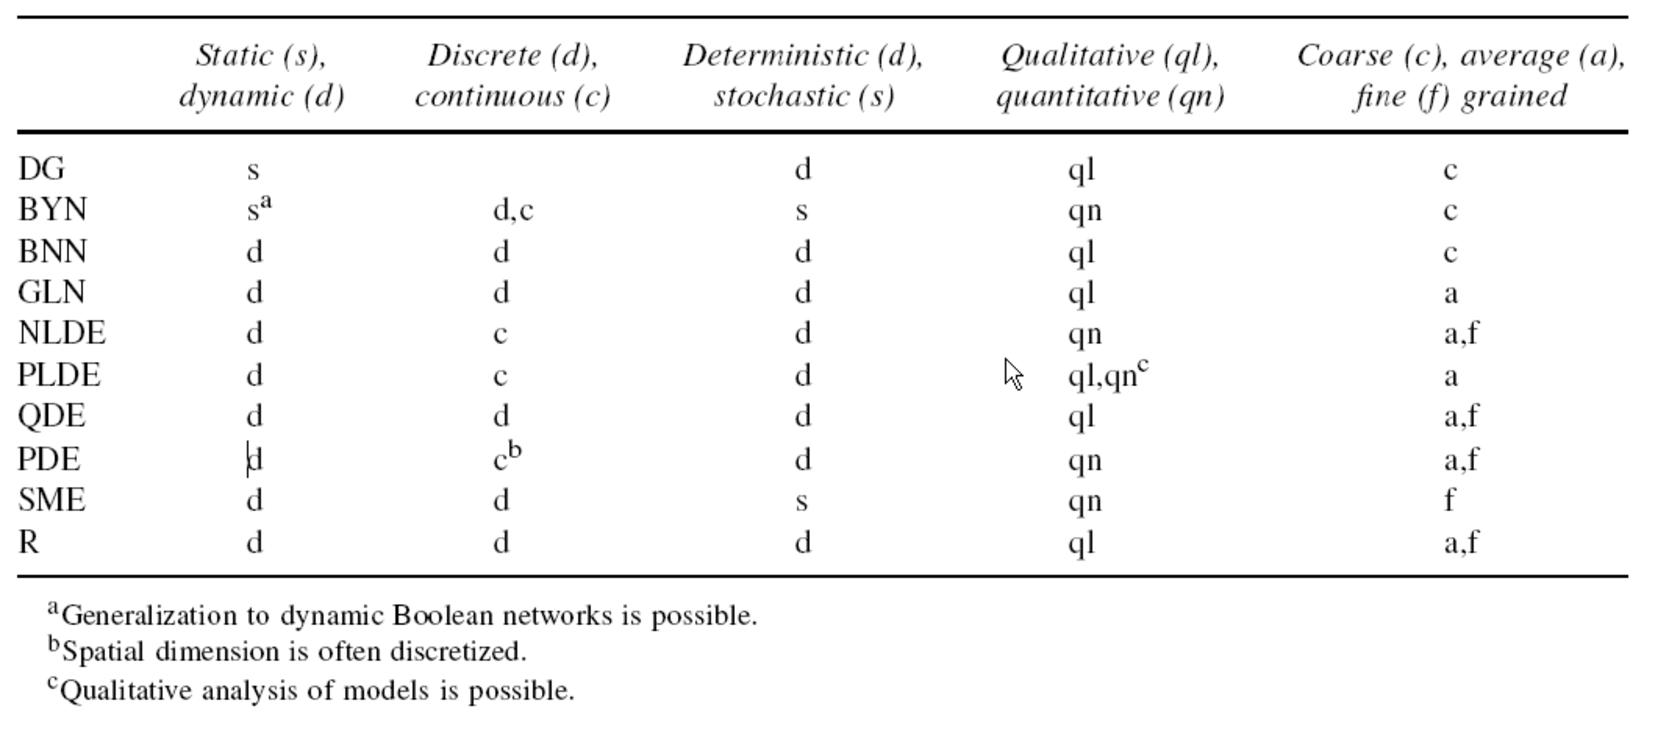
\includegraphics[width=1.00\linewidth]{graphics/graphicastable}  
\end{table}

The same (simplified) table using the \LaTeX\ table feature is shown below (\Cref{tab:latextable}).

\begin{table}[htb]
	\centering
	\caption{Summary of properties of different modelling formalisms. The table below is produced using \LaTeX's {\tt table} environment.}
	\label{tab:latextable}
	\begin{tabular}{cccccc}
		\hline
		& Static & Discrete & Deterministic & Qualitative & Coarse \\
	    \hline
	    DG & s &  & d & ql & c \\
	    BYN & s & d,c & s & qn & c\\
	    BNN & d & d & d & ql & c\\
	    GLN & d & c & d & qn & a,f\\
		\hline
	\end{tabular}
\end{table}

\subsubsection*{A.4.4. Figures}
\label{sec:appendix-a44-figures}

Good figures/diagrams are even more difficult to produce than tables. Figures should contain legends explaining the symbols in the figure. Avoid surrounding the figure with a box outline. If there are different parts of a figure (e.g., (a), (b), (c)), indicate these clearly. Make sure that the labels within a figure/diagram are spelled consistently within the figure/diagram and are also consistently spelled in the text. Make sure that caption appears on the same page as the figure. The figure caption is below the figure. See an example of a figure and its caption below (\Cref{fig:figure}).

Each figure must be introduced in the deliverable text. Make sure that cross references to figures are correct before submitting the deliverable.

The figure caption should follow the sentence style layout and end with a full stop. The figure caption as well as the figure should be centred.

\begin{figure}[htb]
	\centering
	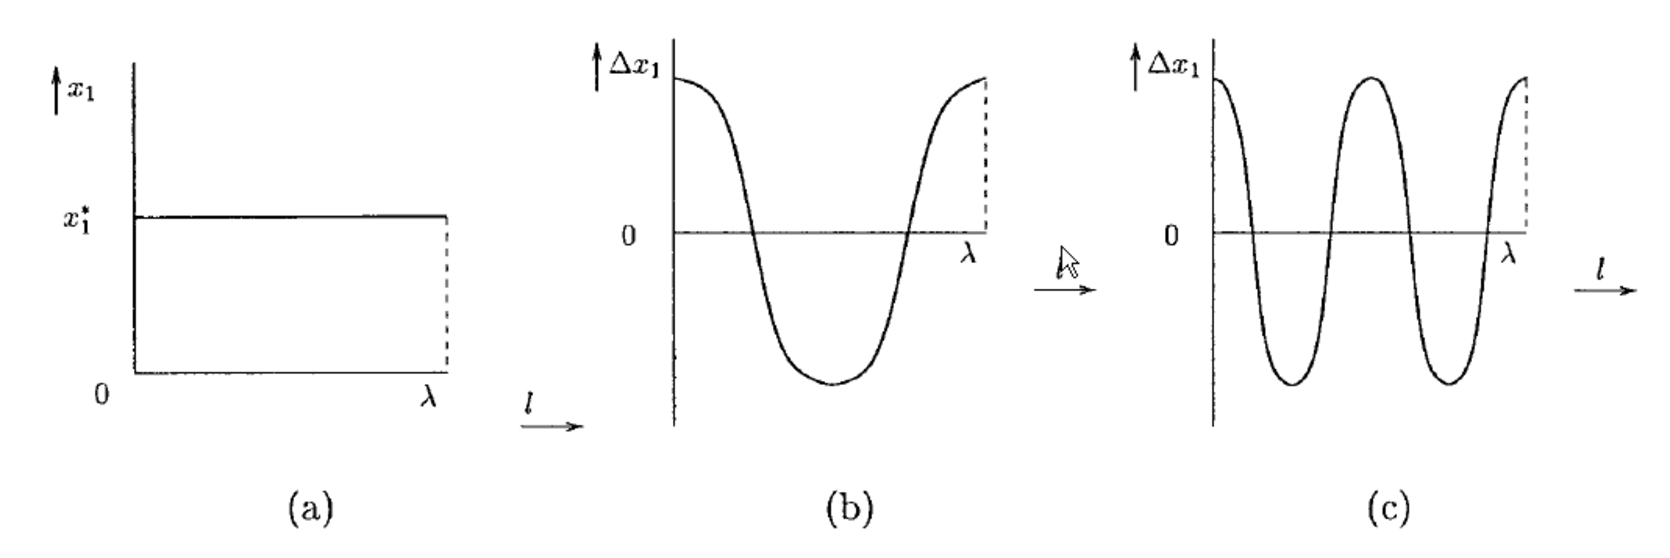
\includegraphics[width=.89\linewidth]{graphics/figure}
	\caption{Caption caption caption caption caption caption caption caption caption. (a) Caption caption caption, (b) Caption caption caption, (c) Caption caption caption.}
	\label{fig:figure}
\end{figure}

\subsubsection*{A.4.5. Footnotes}
\label{sec:appendix-a45-footnotes}

This\footnote{The footnote is at the bottom of the same page where the footnote is cited and the font size is only 9 pt. Footnotes are useful to for including nasty-looking long Web references which would look terrible if used in the main flow of the text.} is a footnote.

\subsection*{A.5. Language and Notation}
\label{sec:appendix-a5-language-notation}
\addcontentsline{toc}{subsection}{A.5. Language and Notation}

There are a few things we should consider when writing documents in terms of language. The question is not deeply philosophical in the sense of whether one or the other approach is fundamentally correct (or wrong). It is more the case of maintaining a certain level of consistency across the project.

Since British/UK English is the official version of English within the EC, we should by default use UK English spelling (and adopt a spell-checker set to UK English). Nevertheless, US spelling is also fine – the main issue to ensure is to be consistent within a given deliverable.

Quotation marks. UK English (unlike US), use single quotation marks (‘X’) instead of double quotation marks (``X''). At least maintain consistency within a document. 

\begin{itemize}
    \item It is claimed that Y is ‘superior’ to X. 
    \item ‘Good morning, Dave,’ greeted HAL.
\end{itemize}

Do not use quotation marks to indicate emphasis – use italics, bold or underline style instead.

The accepted standard for separating orders of magnitude in large figures is not ‘,’ or ‘’’ (quotation mark) or ‘.’, but a non-breaking (small) space. 

\begin{itemize}
    \item This is inappropriate: 1,000,000 or 1.000.000 or 1’000’000 (very bad!) 
    \item This is good: $1\,000\,000$. 
\end{itemize}

Capitalisation. Use capitalisation according to English grammar rules. If someone is interested, see 
capitalisation rules:\footnote{\url{http://andromeda.rutgers.edu/~jlynch/Writing/c.html}, \url{http://www.grammarbook.com/punctuation/capital.asp}}

Tense. Use past tense when describing activities and tasks (experiments, developments, etc) carried out in the past. 

\begin{itemize}
    \item A test bed was set up to ...
    \item The evaluation revealed that ...
\end{itemize}

Use present tense when describing the ideas, design, systems, etc. that exist in the present. 

\begin{itemize}
    \item The system supports the following exchange formats ...
    \item A key property of the system is its ability to ...
\end{itemize}

Large numbers. Use explicit format or scientific notation for large numbers

\begin{itemize}
    \item Use $1\,200\,000\,000$, not 1.2bn or 1,200,000,000
    \item Or use $1.20\,10^9$ or $1.20 \times 10^9$
\end{itemize}

Small numbers. As usual, unless in tables and similar elements, use {one, two, ... , twelve} for numbers < 13, and {13, 14, ..., } for large numbers.

Numbers and units. Use small space (In \LaTeX: \, or ~) to separate figures from units. E.g.,

\begin{itemize}
    \item 10~GB, not 10GB
    \item 2.13~s not 2.13s
\end{itemize}

Bits, bytes and pieces. Use the following terms and abbreviations for bytes (sometimes it is better to use the full term than the abbreviation).

Bits:\\
\begin{tabular}{lll}
    kb or Kb&	kilobit&	103\\ 
    Mb&	megabit&	106\\ 
    Gb&	gigabit&	109\\ 
    Tb&	terabit&	1012\\ 
\end{tabular}

Bytes:\\
\begin{tabular}{lll}
    kB or KB&	kilobyte&	103\\ 
    MB&	megabyte&106\\ 
    GB	&gigabyte	&109\\ 
    TB	&terabyte	&1012\\ 
\end{tabular}

Number of decimals. When a number is expressed in the scientific notation, the number of significant digits (or significant figures) is the number of digits needed to express the number to within the uncertainty of calculation. For example, if a quantity is known to be 1.234 ± 0.002, four figures would be significant\footnote{\url{http://mathworld.wolfram.com/SignificantDigits.html}}.

Unless there is a good reason, do not use more than three fractional digits or places (the number of digits following the point).

Other issues. Avoid overly long sentences. Certain rules suggest that sentence over approximately 20 words become difficult to understand and should therefore be avoided. 

\subsection*{A.6. \LaTeX\ Style Files}
\label{sec:appendix-a6-latex-style-files}
\addcontentsline{toc}{subsection}{A.6. \LaTeX\ Style Files}

\newcommand{\macro}[1]{{\tt \textbackslash #1}}

To use the latex template, copy the contents of this directory and use {\tt template.tex} as the master file of your deliverable (after renaming it as required). The necessary files are:

\begin{itemize}
    \item erigrid2.sty
    \item istcover.sty
    \item istprog.sty
    \item graphics/
    \begin{itemize}
        \item erigrid2-coverbkg.pdf
        \item erigrid2-logo.pdf
        \item erigrid2-partners.pdf
    \end{itemize}
\end{itemize}

Use the following macros to populate the tables on the cover and on page two:

\begin{itemize}
    \item \macro{istChange\{\}\{\}\{\}\{\}}: for setting change log items. The first argument is the date, the second is the deliverable's version number, the third, the author's name, and the   fourth the summary of changes made. You may add as many of these   commands as you like. They will be stored and added to the table on   the second page.  
    \item \macro{ProjectAcronym\{\}}, \macro{ProjectFullTitle\{\}}, \macro{ProjectRefNo\{\}}: these are pre-set to the obvious values. 
    \item \macro{delivNumber\{\}}: the deliverable number, Dx.y
    \item \macro{delivName\{\}}: deliverable's title, as appears in the DoA
    \item \macro{delivShortTile\{\}}: Short Title
    \item \macro{delivResponsible\{\}}: partner in charge of the deliverable
    \item \macro{delivVersion\{\}}: version as vn.n
    \item \macro{ActualDate\{\}}: date of submission
    \item \macro{delivDissLevel\{\}}: PU, PP, RE or CO
    \item \macro{delivType\{\}}: R = report or O = other
    \item \macro{delivWP\{\}}: not used
    \item \macro{delivAuthor\{\}}: Lead author(s)
    \item \macro{delivFPAuthor\{\}}: Co-author(s)
    \item \macro{delivStatus\{\}}: (d)raft, (f)inal, or (s)ubmitted
    \item \macro{delivKeywords\{\}}: well...
\end{itemize}

These declarations must appear before you issue the \macro{makecover} command, at the beginning of the report.

\subsection*{A.7. Formatting Bibliographical References}
\label{sec:appendix-a7-formatting-bibliographical-references}
\addcontentsline{toc}{subsection}{A.7. Formatting Bibliographical References}

By default, references should use APA style (as, e.g., used in Google Scholar) and be ordered in alphabetic order. See for example \cite{bib:tan2004}, in the list below.

Other styles are also OK, nevertheless the authors should make sure that within a single document the notation to references and their citation should be consistent. In the text, the references should ideally be referred to by the author name and year, e.g., \cite{bib:lamport1994}; however, referencing by reference number is also acceptable.

\subsection*{A.8. Associated Outputs}
\label{sec:appendix-a8-associated-outputs}
\addcontentsline{toc}{subsection}{A.8. Associated Outputs}

\textit{If appropriate, please include a section with details of any datasets, code or other resources being released with this deliverable.}

The work described in this deliverable has resulted in the following resources:

\begin{center}
    \def\arraystretch{1.25}		
    \begin{tabular}{|c|c|c|}
        \hline
        \rowcolor{erigrid2gray}
        \color{white} Description & 
        \color{white} URL & 
        \color{white} Availability 
        \\\hline
    
        \rowcolor{white}\color{erigrid2font} 
        My Dataset 1 &  
        \url{http://hdl.handle.net/12345} &
        Public (Apache 2.0) \\
    
        \rowcolor{erigrid2lightergray}\color{erigrid2font} 
        My Dataset 2 &  
        \url{http://hdl.handle.net/54321} &
        Private (consortium only) \\
    
        \rowcolor{white}\color{erigrid2font} 
        My Code &  
        \url{github.com/erigrid2/xxx} &
        Public (GPL3) \\
    
        \hline
    \end{tabular}
\end{center}

%%%%%%%%%%%%%%%%%%%%%%%%%%%%%%%%%%%%%%%%%
%%%%%%%%%%%%%%%%%%%%%%%%%%%%%%%%%%%%%%%%%
%%% Appendix B
%%%%%%%%%%%%%%%%%%%%%%%%%%%%%%%%%%%%%%%%%

\clearpage
\section*{Appendix B}
\addcontentsline{toc}{section}{Appendix B}
\label{sec:appendix-b}

%%%%%%%%%%%%%%%%%%%%%%%%%%%%%%%%%%%%%%%%%
%%% Section content, please change!
%%%%%%%%%%%%%%%%%%%%%%%%%%%%%%%%%%%%%%%%%

\subsection*{Appendix B.1}
\label{sec:appendix-b1}
\addcontentsline{toc}{subsection}{Appendix B.1}

\todo{Explain the content of the appendix.}

\subsection*{Appendix B.2}
\label{sec:appendix-B2}
\addcontentsline{toc}{subsection}{Appendix B.2}

\todo{Explain the content of the appendix.}

%%%%%%%%%%%%%%%%%%%%%%%%%%%%%%%%%%%%%%%%%
%%%%%%%%%%%%%%%%%%%%%%%%%%%%%%%%%%%%%%%%%
%%% Appendix C
%%%%%%%%%%%%%%%%%%%%%%%%%%%%%%%%%%%%%%%%%

\clearpage
\section*{Appendix C}
\addcontentsline{toc}{section}{Appendix C}
\label{sec:appendix-c}

%%%%%%%%%%%%%%%%%%%%%%%%%%%%%%%%%%%%%%%%%
%%% Section content, please change!
%%%%%%%%%%%%%%%%%%%%%%%%%%%%%%%%%%%%%%%%%

\subsection*{Appendix C.1}
\label{sec:appendix-c1}
\addcontentsline{toc}{subsection}{Appendix C.1}

\todo{Explain the content of the appendix.}

\subsection*{Appendix C.2}
\label{sec:appendix-c2}
\addcontentsline{toc}{subsection}{Appendix C.2}

\todo{Explain the content of the appendix.}

%%%%%%%%%%%%%%%%%%%%%%%%%%%%%%%%%%%%%%%%%

%%%%%%%%%%%%%%%%%%%%%%%%%%%%%%%%%%%%%%%%%
%%% Back Page
%%%%%%%%%%%%%%%%%%%%%%%%%%%%%%%%%%%%%%%%%

\makedisclaimer

\end{document}

%%%%%%%%%%%%%%%%%%%%%%%%%%%%%%%%%%%%%%%%%
